\documentclass{article}
\usepackage{graphicx} % Required for inserting images
\usepackage[utf8]{inputenc}
\usepackage[T1]{fontenc}
\usepackage{karnaugh-map}
\usepackage[polish]{babel}
\usepackage{subcaption}
\usepackage{float}
\usepackage{enumitem}
\usepackage{url}


\begin{document}
	\begin{center}
	%\includegraphics[scale=0.35]{logo.png}	
	
	\textbf{Sprawozdanie z Laboratorium} \\
	\vspace{0.1cm}\
	\textbf{Modułowe systemy cyfrowe}
	\vspace{0.1cm}\
	\end{center}	

\noindent Wykonujący ćwiczenie: Kamil Kubajewski, Bartosz Orłowski, Jakub Matusiewicz \\
\vspace{3cm} \\
Studia dzienne I stopnia \\
Kierunek: Informatyka \\
Semestr: II \hspace{4cm} Grupa zajęciowa: LAb 8 \\
\\
Prowadzący ćwiczenie: \textbf{...} \\
\phantom{a} \hfill .................. \\
\phantom{a} \hfill OCENA \\
\\ 
\vfill \noindent
Data wykonania ćwiczenia \\
15 października 2025 r.\ \\
\phantom{a} \hfill ............................................\\
\phantom{a} \hfill Data i podpis prowadzącego

\pagebreak
\begin{center}
    \hspace{-1.2cm}
    \begin{tabular}{|p{0.7\textwidth}|l|}
        \hline
        Wydział Informatyki Politechniki Białostockiej \hfill & Data: 15.10.2025 \\
        Przedmiot: Modułowe systemy cyfrowe \hfill & \\
        \hline
        Zajęcia nr 2 & Prowadzący: \\
        Temat: Parametry statyczne i dynamiczne bramek oraz przerzutników & \textbf{...}\phantom{Phantom Phantomphantom} \\
        & \\
        Grupa: Lab 8 & \\
        Imię i nazwisko: & \\
        Kamil Kubajewski, Bartosz Orłowski, Jakub Matusiewicz & \\
        \hline
    \end{tabular}
\end{center}

\section{Cel ćwiczeń}

Zapoznanie z podstawowymi parametrami wybranych układów cyfrowych TTL, konkretnie z przerzutnikami \textbf{ D, T, RS} oraz \textbf{JK}.

\section{Podstawa teoretyczna}
    Na zajęciach będziemy zajmować się bramkami logicznymi i przerzutnikami, które stanowią elementy elektroniki cyfrowej. Bramki logiczne odpowiadają za operacje logiczne, natomiast przerzutniki umożliwiają przechowywanie i przełączanie stanów logicznych w odpowiedzi na sygnały zegarowe.

    \subsection{Bramki TTL}
    Bramki logiczne TTL( Transistor Transistor Logic) stanowią rezultat ewolucji oraz doskonalenia bipolarnych technologii przewodnikowych. 
    Pierwsza bramka TTL powstała dzięki pracy Jamesa L. Buie'a z TRW Inc. w 1961 roku, a już w 1963 roku trafiły one do sprzedaży za pomocy firmy Sylvania, które były początkowo wykorzystywane do celów militarnych\cite{maciak,wiki}.\\
   
    Największa popularność zyskały wsród projektantów urządzeń elektronicznych TTL w amerykańskim przedsiębiorstwie Texas Instruments. To oni są odpowiedzielani za rodzinę układów 7400 wprowadzoną w 1964 roku do masowej produkcji cyfrowych układów scalonych i jest ona wykorzystywana do dzisiaj\cite{maciak,wiki,TI7400}. \\
    
    Układy typu TTL zbudowane są z tranzystorów bipolarnych i są one zasilane napięciem stałym 5V. Działają one w logice dodatniej, czyli stan niski ( logiczne "0"), czyli 0V oraz stan wysoki( logiczne "1") odpowiadające 5V. W rzeczywistych warunkach napięcia te mogą jednak odbiegać od wartości idealnych z powodu niedoskonałości elementów i ograniczeń technologicznych\cite{maciak,wiki,TI7400}.
    \pagebreak
    
    Bramki konstruowane są w taki sposób, aby stan logiczny na wyjściu posiadał pewien zapas w stosunku do wymaganych napięć na wejściu\cite{TI7400}. Dzięki temu zapewniona jest poprawna praca układu i odporność na zakłócenia, dlatego:
    \begin{itemize}
        \item Logiczna 1 to stan wysoki, w którym napięcie ma wartość od 2.4V do 5V.
        \item Logiczna 0 to stan niski, w którym napięcie wynosi 0V, ale może wahać się między 0V do 0.4V.
        \item Dodatkowo bramka TTL posiada tzw. margines odporności na zakłócenia, wynoszący około 0.4V zarówno na wejściu i wyjściu bramki.
        \begin{figure}[h]
        	\centering
        	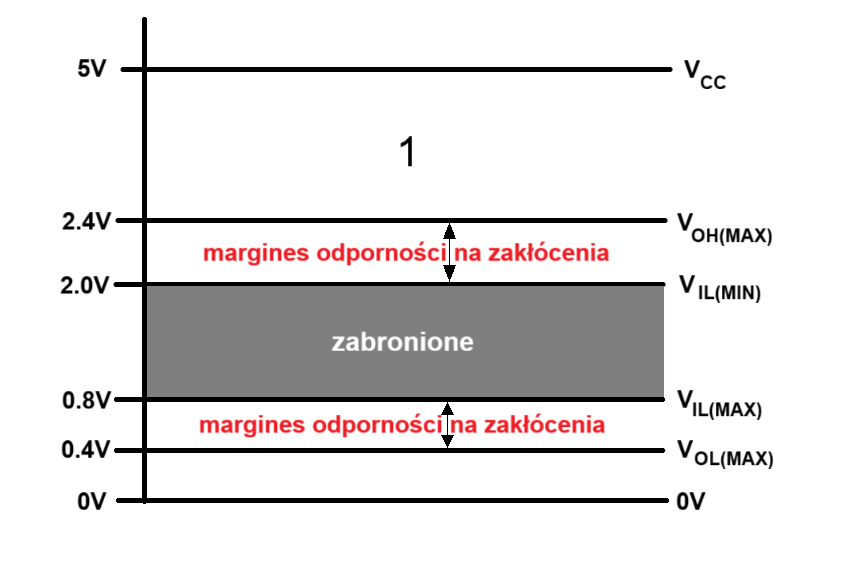
\includegraphics[width=0.8\textwidth]{margines.PNG}
        	\caption{Wykres napięć bramki TTL wraz z marginesami zakłóceń}
        	\label{fig:moj_obrazek}
        \end{figure}
        \item Czasy tpHL, tpLH: są to czasy potrzebne do zmiany stanu logicznego na wyjściu bramki: 
        \begin{itemize}
            \item tpHL – czas, w którym sygnał logiczny zmienia się z poziomu wysokiego na niski stan,
            \item tpLH – czas, w którym sygnał logiczny zmienia się z poziomu niskiego na wysoki stan.
        \end{itemize}
    \end{itemize}
    
    \begin{figure}[h]
    	\centering
    	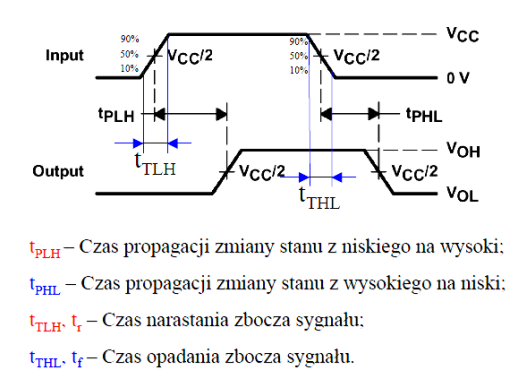
\includegraphics[width=0.6\textwidth]{czas.PNG}
    	\caption{Wykres czasowy dynamicznej zmiany stanu bramki( Maciak, 2021 [1])}
    	\label{fig:moj_obrazek}
    \end{figure}

	\pagebreak
	
    \subsection{ Przerzutniki}

    Przerzutniki to układy, które pozwalają na przechowywanie jednego bitu informacji. Używane są w licznikach, rejestrach, pamięciach oraz innych układach wymagających przechowywania stanów logicznych\cite{wiki-flip}.

    \subsubsection{Przerzutnik typu D}
    \begin{table}[H]
    	\centering
    	\begin{tabular}{|c|c|c|}
    		\hline
    		\textbf{Q$_i$} & \textbf{D} & \textbf{Q$_{i+1}$} \\ \hline
    		0 & 0 & 0 \\ 
    		0 & 1 & 1 \\ 
    		1 & 0 & 0 \\ 
    		1 & 1 & 1 \\ 
    		\hline
    	\end{tabular}
    	\caption{Tabela wzbudzeń przerzutnika typu D}
    \end{table}
    
    \subsubsection{Przerzutnik typu JK}
    \begin{table}[H]
    	\centering
    	\begin{tabular}{|c|c|c|c|}
    		\hline
    		\textbf{Q$_i$} & \textbf{J} & \textbf{K} & \textbf{Q$_{i+1}$} \\ \hline
    		0 & 0 & - & 0 \\ 
    		0 & 1 & - & 1 \\ 
    		1 & - & 1 & 0 \\ 
    		1 & - & 1 & 1 \\ 
    		\hline
    	\end{tabular}
    	\caption{Tabela wzbudzeń przerzutnika typu JK}
    \end{table}
    
    \subsubsection{Przerzutnik typu T}
    \begin{table}[H]
    	\centering
    	\begin{tabular}{|c|c|c|}
    		\hline
    		\textbf{Q$_i$} & \textbf{T} & \textbf{Q$_{i+1}$} \\ \hline
    		0 & 0 & 0 \\ 
    		0 & 1 & 1 \\ 
    		1 & 0 & 1 \\ 
    		1 & 1 & 0 \\ 
    		\hline
    	\end{tabular}
    	\caption{Tabela wzbudzeń przerzutnika typu T}
    \end{table}
    
    \subsubsection{Przerzutnik typu SR (Set-Reset)}
    \begin{table}[H]
    	\centering
    	\begin{tabular}{|c|c|c|}
    		\hline
    		\textbf{R} & \textbf{S} & \textbf{Q$_i$} \\ \hline
    		0 & 0 & Q$_{i-1}$ \\ 
    		0 & 1 & 1 \\ 
    		1 & 0 & 0 \\ 
    		1 & 1 & N \\ 
    		\hline
    	\end{tabular}
    	\caption{Tabela wzbudzeń przerzutnika typu SR}
    \end{table}
    

    \pagebreak

\pagebreak
\section{Przebieg ćwiczeń}
\subsection{Zadanie 1}
W układzie jak na rysunku zdjąć powierzchnię charakterystyczną bramki 7400. Układ
scalony 7400 umieścić w podstawce modułu DB26.

\begin{figure}[h]
    \centering
    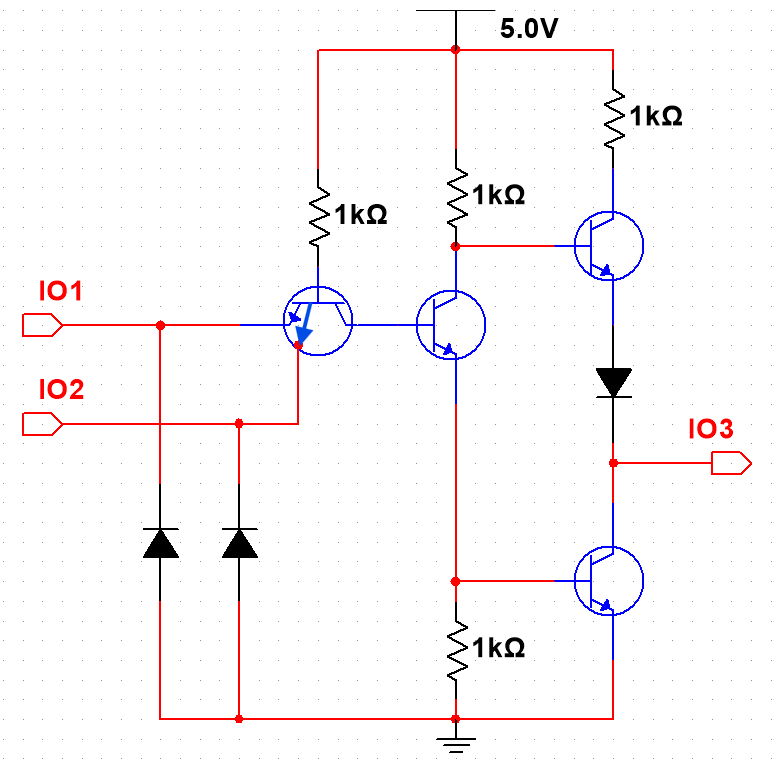
\includegraphics[width=0.8\textwidth]{obwod1.PNG}
    \caption{Bramka NAND}
    \label{fig:moj_obrazek}
\end{figure}
%\textbf{modułu DB11} przerzutniki

Do przetestowania i dokonania pomiarów użyto \textbf{modułu DB26} do którego wpięto \textbf{układ scalony 7400}, czyli bramka \textbf{NAND}. Do pomiarów dla wejśc podłączono zasilanie (5 V jako jedynka logiczna i 0 V jako zero logiczne), które było regulowane, sprawdzić otrzymane napięcie na wyjściu. Daje to poniższe pomiary(tabela 1):
\pagebreak
\begin{table}[!ht]
    \centering
    \caption{Pomiary dla rożnych danych wejść}
    \begin{tabular}{|l|l|l|}
    \hline
        V\_1 [V] & V\_2 [V] & Output[V] \\ \hline
        5,00 & 5,00 & 0,0645 \\ \hline
        4,50 & 5,00 & 0,0645 \\ \hline
        4,00 & 5,00 & 0,0645 \\ \hline
        3,50 & 5,00 & 0,0645 \\ \hline
        3,00 & 5,00 & 0,0645 \\ \hline
        2,50 & 5,00 & 0,0645 \\ \hline
        2,00 & 5,00 & 0,0645 \\ \hline
        1,50 & 5,00 & 0,0645 \\ \hline
        1,00 & 5,00 & 2,5410 \\ \hline
        0,50 & 5,00 & 3,7430 \\ \hline
        0,30 & 5,00 & 3,9290 \\ \hline
        5,00 & 4,50 & 0,0645 \\ \hline
        5,00 & 4,00 & 0,0645 \\ \hline
        5,00 & 3,50 & 0,0645 \\ \hline
        5,00 & 3,00 & 0,0645 \\ \hline
        5,00 & 2,50 & 0,0645 \\ \hline
        5,00 & 2,00 & 0,0645 \\ \hline
        5,00 & 1,50 & 0,0645 \\ \hline
        5,00 & 1,00 & 3,1890 \\ \hline
        5,00 & 0,50 & 3,9060 \\ \hline
        5,00 & 0,30 & 3,9320 \\ \hline
        1,20 & 3,70 & 2,5800 \\ \hline
        3,70 & 1,20 & 2,5500 \\ \hline
        3,10 & 0,80 & 3,4050 \\ \hline
        0,80 & 3,10 & 3,5010 \\ \hline
        1,20 & 2,80 & 2,4110 \\ \hline
        2,80 & 1,20 & 2,5620 \\ \hline
        2,80 & 2,40 & 0,0647 \\ \hline
        2,40 & 2,80 & 0,0647 \\ \hline
        1,60 & 1,20 & 2,7020 \\ \hline
        1,20 & 1,60 & 2,5330 \\ \hline
    \end{tabular}
\end{table}
\pagebreak

\begin{figure}[h]
    \centering
    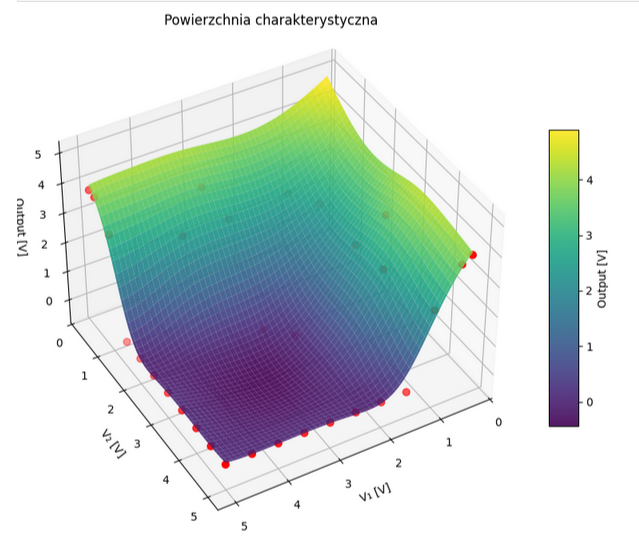
\includegraphics[width=0.5\textwidth]{powierzchnia.PNG}
    \caption{Wykres powierzchni charakterystycznej}
    \label{fig:moj_obrazek}
\end{figure}

\subsection{Zadanie 3}
W zadaniu 3 przetestowano działanie przerzutników \textbf{T, RS, JK, D} za pomocą \textbf{modułu DB11}. Poniżej zamieszczone są schematy poszczególnych przerzutników.

\begin{figure}[h]
    \centering
    \begin{subfigure}[t]{0.3\textwidth}
        \centering
        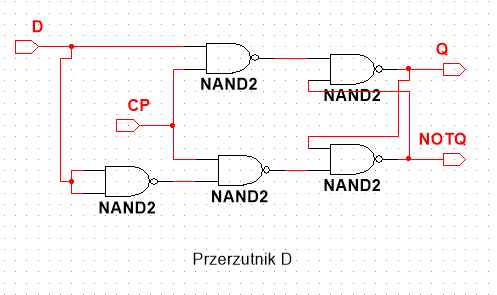
\includegraphics[width=\textwidth]{D.png}
        \caption{Schemat przerzutnika D}
    \end{subfigure}
    \hfill
    \begin{subfigure}[t]{0.3\textwidth}
        \centering
        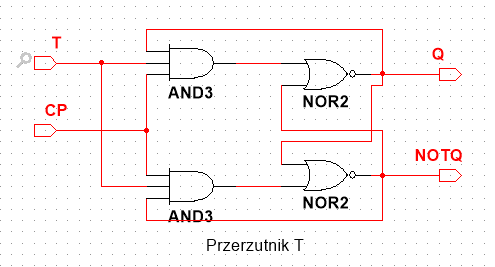
\includegraphics[width=\textwidth]{T.png}
        \caption{Schemat przerzutnika T}
    \end{subfigure}
    \hfill
    \begin{subfigure}[t]{0.3\textwidth}
        \centering
        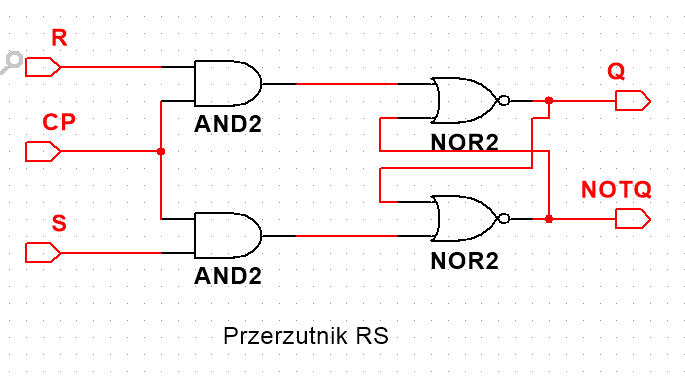
\includegraphics[width=\textwidth]{RS.png}
        \caption{Schemat przerzutnika RS}
    \end{subfigure}
        \hfill
    \begin{subfigure}[t]{0.3\textwidth}
        \centering
        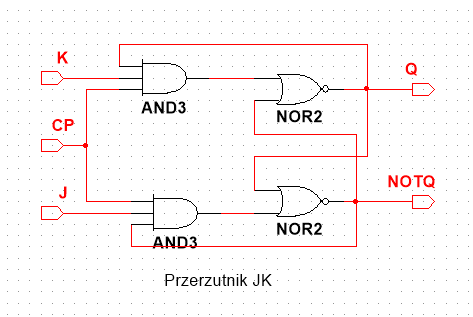
\includegraphics[width=\textwidth]{JK.png}
        \caption{Schemat przerzutnika JK}
    \end{subfigure}
    \caption{Schematy przerzutników JK, RS, T, D}
    \label{fig:bramki}
\end{figure}

\pagebreak
\section{Dyskusja błedów}
%Klasyczna formułka np. z EDI, jaka powinna byc oczekiwana wartość? Bład ludzki, niedokładnosc przyrządów, itd

W zadaniu pierwszym badano powierzchnie charaketrystyczną bramki 7400. Podawane napięcia na wejścia bramki NAND wynosiły od 0V do 5V. W zależności od podanych napięć na wejściach otrzymywano różne napięcia na wyjściu. Dla stanu niskiego ( logiczne "0") napięcie wyjściowe zawierało się w przedziale od 0,0645 V do 0,0647 V. Aby obliczyć procentowe odchylenie wartości rzeczywistej od wartości teoretycznej, trzeba przyjąć maksymalne napięcie dla stanu wysokiego( 0,4V) oraz średnią wartość wszystkich napięć dla stanu niskiego odjętą o maksymalne napięcie wyjściowe dla stanu wyoskiego:
\begin{center}
	$\frac{|0,0646V-0,4V|}{0,4V}$ $\ast$ 100\% $\approx$ 83,85\%
\end{center}

Napięcie stanu wysokiego ( logiczne "1") wahał się od 2,4110V do 3,9320V. Aby obliczyć procentowe odchylenie rzeczywistej od wartości teoretycznej, trzeba przyjąć minimalne napięcie dla stanu wysokiego( 2,4V) oraz średnią wartość wszystkich napięć dla stanu wysokiego odjętą o minimalne napięcie wyjściowe dla stanu wyoskiego:
\begin{center}
	$\frac{|3,106V - 2,4V|}{2,4V}$ $\ast$ 100\% $\approx$ 29,42\%
\end{center}

Uzyskane wartości napięć różnią się od teoretycznych o ok. 84\% dla stanu niskiego oraz 29\% dla stanu wysokiego.
Mimo dużej różnicy procentowej, obie wartości mieszczą się w dopuszczalnych granicach teoretycznych, co oznacza, że bramka 7400 pracuje poprawnie i zachowuje właściwą logikę stanów.\linebreak

Różnice te mogą wynikać z następujących przyczyn:

\begin{itemize}
	\item Dokładność użytego przyrządu pomiarowego, którego błąd pomiarowy przyjęto na potrzeby tych pomiarów jako 0.7V.
	\item Spadki napięć na tranzystorach wewnętrznych układu, które wynikają z ich charakterystyki półprzewodnikowej.
	\item Tolerancja elementów wewnętrznych.
\end{itemize}

W zadaniu trzecim wyniki rzeczywiste nie różnią się od wartości teoretycznych. Pomiary wykazane na rzeczywistych układach odpowiadają tym w tablicach wzbudzeń dla konkretnych przerzutników.

\section{Wnioski}
W naszych zadaniach można było zaobserwować zachowanie bramek TTL, przerzutników D, T, RS oraz JK. W zadaniu pierwszym zbadano powierzchnie charakterystyczną bramki 7400 poprzez zmianę napięć na wejścia oraz pomiar napięcia na wyjściu. Otrzymane wyniki potwierdziły, że stany napięć logicznych nie są idealnie równe 0V( logiczne "0") oraz 5V( logiczne "1"), co jest zgodne z teorią działania brmake TTL. Dodatkowo zaobserwowano również margines odporności na zakłócenia, które zapewniają interpretację stanów logicznych pomimo niewielkich odchyleń napięć. Dzięki temu można było zaobserować rzeczywistą, nieliniową charakterystykę przejścia pomiędzy stanami logicznymi.\\

W zadaniu trzecim zaobserwowano rzeczywiste działanie przerzutników. Pozwoliło na zweryfikowanie tablic wzbudzeń przerzutników D, T, JK oraz RS, co jest zgodne z teorią działania układów sekwencyjnych.
\pagebreak
\section{Literatura}

\renewcommand{\refname}{}

\begin{thebibliography}{9}
	
	\bibitem{maciak} 
	T. Maciak, \textit{Skrypt do laboratorium Elektroniki cyfrowej}, 
	Wydział Informatyki Politechniki Białostockiej, Białystok, 2021.
	
	\bibitem{wiki} 
	\textit{Transistor–transistor logic}, Wikipedia, dostęp online: 
	\url{https://en.wikipedia.org/wiki/Transistor-transistor_logic}, 
	data dostępu: październik 2025.
	
	\bibitem{wiki-flip} 
	\textit{Excitation table}, Wikipedia, dostęp online: 
	\url{https://en.wikipedia.org/wiki/Excitation_table}, 
	data dostępu: lipiec 2025.
	
	\bibitem{TI7400} 
	Texas Instruments, \textit{SN7400 NAND Gate Datasheet}, dostęp online: 
	\url{https://www.ti.com/lit/ds/symlink/sn7400.pdf}, 
	data dostępu: 2017.
	
\end{thebibliography}

\pagebreak
\section{Protokół}

\begin{figure}[h]
    \centering
    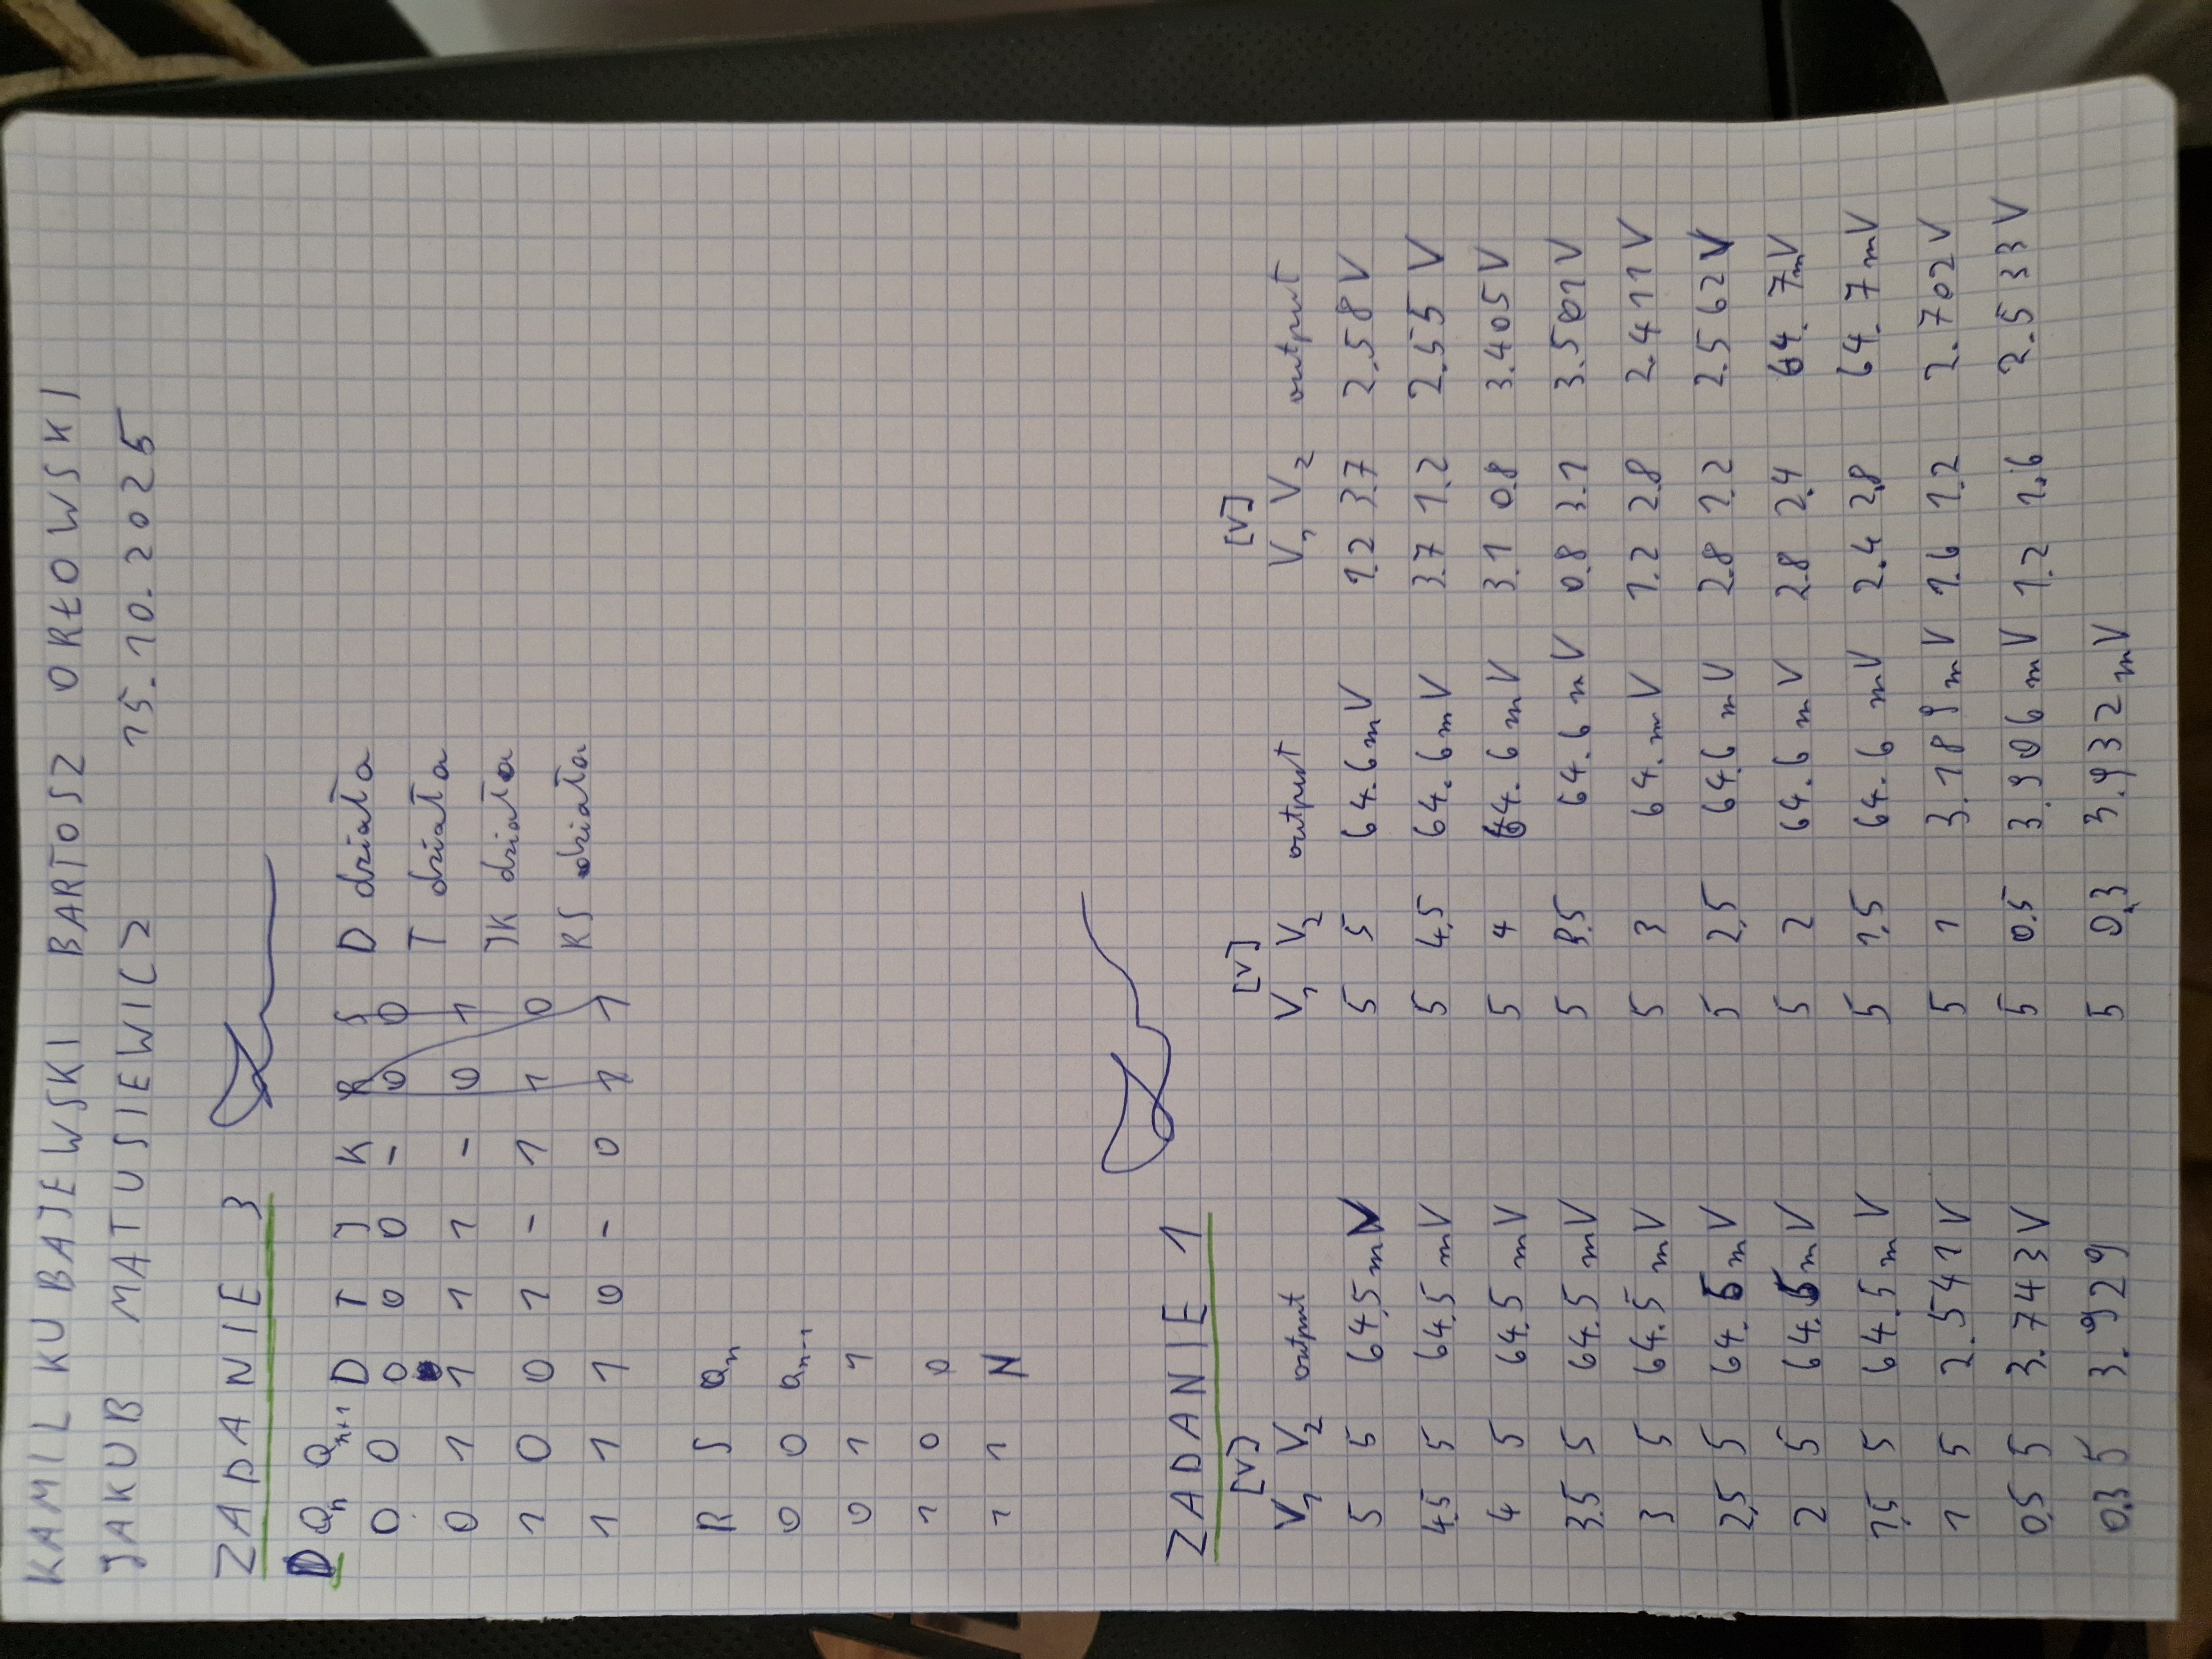
\includegraphics[width=0.8\textwidth, angle=-90]{protokol.JPG}
    \caption{Protokół}
    \label{fig:moj_obrazek}
\end{figure}
\end{document}
